\documentclass{amsart}

\usepackage{amsmath}
\usepackage{cite}
\usepackage{graphicx}
\usepackage{url}

\newtheorem{theorem}{Theorem}
\newtheorem{lemma}{Lemma}
\newtheorem{corollary}{Corollary}
\newtheorem{proposition}{Proposition}
\newtheorem{example}{Example}
\newtheorem{definition}{Definition}

\newcommand{\RR}{\mathbb R}
\newcommand{\fS}{\mathfrak S}

\newcommand{\aut}{\mathcal A}
\newcommand{\pairing}{\mu}
\newcommand{\tangle}{\mathsf{X}}
\newcommand{\ptree}{\mathsf{P}}
\newcommand{\ptequiv}{\bar{\ptree}}  % Phylogenetic tree equivalence classes under the symmetric group.
\newcommand{\stpair}{\mathsf{Q}}  % Shape-tree pair.
\newcommand{\bigproj}{\tilde \pi}

% arxivness
\newcommand{\arxiv}[1]{#1}
\newcommand{\notarxiv}[1]{}

\newcommand{\FIGspr}{\
\label{FIGspr}
\begin{figure}
  \arxiv{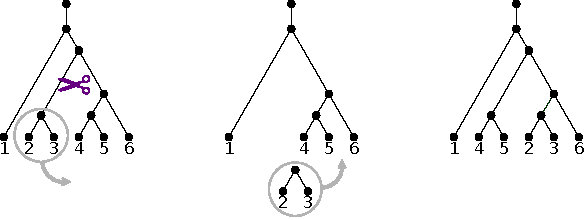
\includegraphics[width=4in]{figures/spr-definition}}
\caption{\
  A subtree-prune-regraft move.
}
\end{figure}
}

\newcommand{\FIGrelabeling}{\
\label{FIGrelabeling}
\begin{figure}
  \arxiv{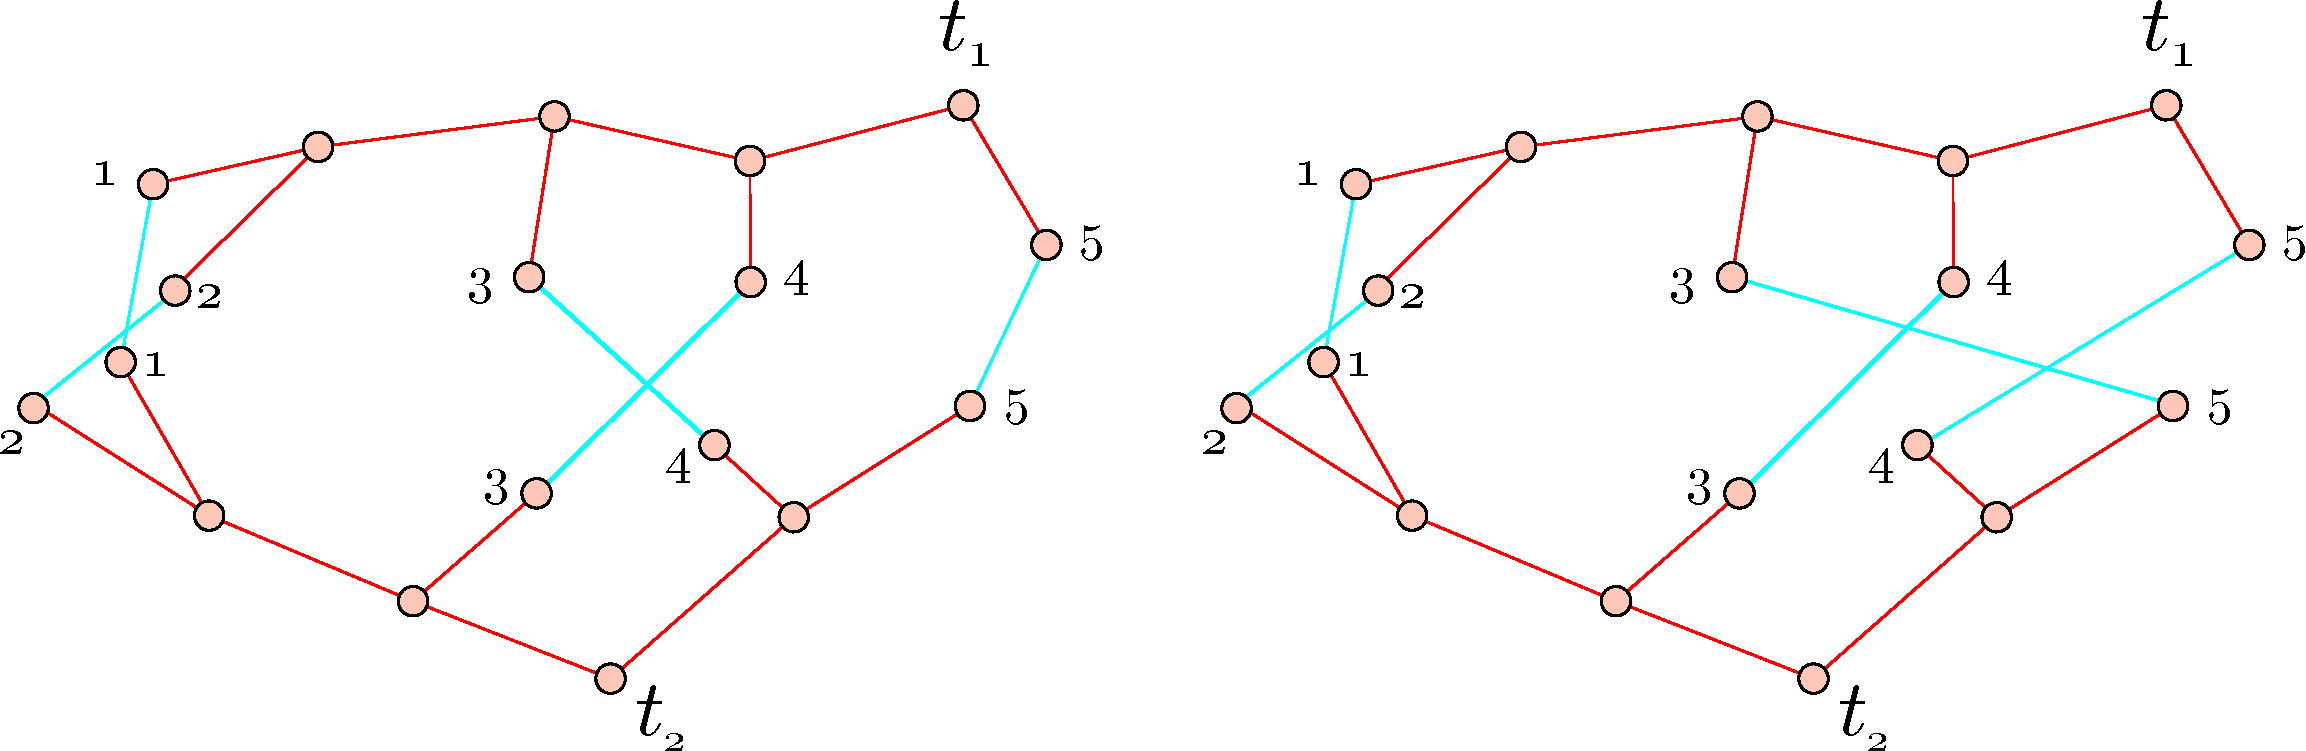
\includegraphics[width=5in]{figures/relabeling-example}}
\caption{\
  A relabeling symmetry (see text for details).
}
\end{figure}
}


\begin{document}
\title{Symmetries of tanglegrams}
\author[Matsen]{Frederick A. Matsen IV}
\address{Fred Hutchinson Cancer Research Center \\ Seattle, WA}
\thanks{Research supported in part by National Science Foundation award 1223057 and National Institutes of Health grant R01 GM113246-01}


\date{\today}

\begin{abstract}
Many interesting discrete mathematics problems concerning phylogenetic trees are defined in terms of the relative labeling of pairs of leaf-labeled trees.
These relative labelings are naturally formalized as so-called ``tanglegrams.''
Although there has been considerable work on planar embeddings of tanglegrams, many questions remain concerning their symmetries.
Understanding symmetries of tanglegrams would give information on how many problems on relatively labeled pairs of trees there are, open up the possibility for amortized algorithms, and reveal natural symmetries of spaces associated with such problems.
In this paper we develop methods to enumerate tanglegrams up to isomorphism, and we investigate the representation of the symmetric group induced by its action on tanglegrams.
\end{abstract}

\maketitle


\section{Introduction}
As a motivating example, we consider the problem of computing the \emph{subtree-prune-regraft} (SPR) distance between two leaf-labeled phylogenetic trees.
An SPR move cuts one edge of the tree and then reattaches the resulting rooted subtree at another edge (Figure~\ref{FIGspr}).
The SPR distance between two (phylogenetic, implying meaning leaf-labeled) trees $t_1$ and $t_2$ is the minimum number of SPR moves required to transform $t_1$ into $t_2$.

Clearly the distance between two such trees does not depend on the actual labels of $t_1$ and $t_2$.
For example, one could exchange numbers labeling the two trees with their corresponding taxonomic names.
Or one could simply permute the numerical labels of the leaf nodes, which would result in the same problem if the permutation was applied identically on both the starting and ending trees.
Furthermore, a path made by SPR moves made by intermediate trees between the two trees could also have its labels permuted in order to give a path between the trees with permuted leaf labels.
Thus, all of these problems do not concern the actual leaf labels as such, but rather use the leaf labels as markers that can be used to map leaves of one phylogenetic tree on to another: the problem and its solutions are actually defined in terms of a \emph{relative} leaf labeling.
\FIGspr

Such discrete mathematics problems and objects defined in terms of pairs of labeled combinatorial objects are ubiquitous in computational biology.
In addition to SPR distances and their cousin distances formed by \emph{nearest-neighbor-interchange} and \emph{tree bisection and reattachment} \cite{wiki:treeRearrangement}, we have their corresponding biological questions concerning ``supertree'' reconstruction \cite{Whidden2014-ku} and reconciliation of gene transfer networks \cite{Boon2013-mc}.
Because such moves are used in both maximum-likelihood heuristic search and Bayesian Markov chain Monte Carlo (MCMC) tree reconstruction, the geometry of phylogenetic trees under such moves has substantial consequences in terms of phylogenetic tree reconstruction \cite{Whidden2014-yt}.

Another line of inquiry in computational biology concerns species delimitation, which can naturally be phrased in terms of inference of a partition of labeled objects.
In an analogous way, scientists use MCMC to explore the posterior on such partitions \cite{Yang2010-kc}, and comparison of the results can be performed using distances between the partitions via distances such as \cite{Gusfield2002-il}.
These partitions can also be thought of as a certain type of leaf-labeled tree of height two, and thus they also form a problem concerning relative leaf labeling of phylogenetic trees.

The concept of a pair of phylogenetic trees with a relative leaf labeling is essentially the same as the graph-theoretic notion of a \emph{tanglegram}.
A tanglegram is a pair of trees on the same set of leaves with matching leaves in the two trees joined by an edge. \cite{Venkatachalam2010-zh}.
There has been extensive work concerning tanglegrams, focusing on the problem of drawing them in a way that has minimum crossings \cite{Buchin2008-lc,Lozano2008-tp,Bansal2009-ni,Bocker2009-xl,Fernau2010-an,Venkatachalam2010-zh}.

In this paper we explore the mapping of pairs of leaf-labeled trees into the set of tanglegrams and explore the action of the symmetric group on tanglegrams.
We characterize the isomorphism classes in terms of the symmetries of the two phylogenetic trees they contain.
Furthermore, tanglegrams are equipped with a natural action of the symmetric group on the leaf set, which we describe.
We use the SAGE \cite{SteinJoyner2005} and GAP \cite{GAP4} mathematics software to further explore these symmetries, resulting in tables of representatives of tanglegrams and their multiplicities, as well as the irreducible representations of the symmetric group defined by the action on tanglegrams.


\section{Formalism}
Define isomorphism of leaf-labeled trees?
versus graph isomorphism.

It will be convenient for our purposes to use a slightly different \emph{labeled} definition of a tanglegram than has been previously used.
Let $\fS_n$ denote the symmetric group on $n$ items.
\begin{definition}
\label{def:tanglegram}
A rooted (resp. unrooted) $n$-\emph{tanglegram} is an ordered triple $(t_1, t_2, \pairing)$ where $t_1$ and $t_2$ are rooted (resp. unrooted) trees with $n$ leaves on the same leaf set, and $\pairing \in \fS_n$ is a permutation of the leaf labels of their common leaf set.
Let $\tangle_n$ denote the set of $n$-tanglegrams.
\end{definition}
\begin{definition}
\label{def:tanglegraph}
A rooted (resp. unrooted) $n$-\emph{tanglegraph} is a graph consisting of two non-leaf-labeled rooted (resp. unrooted) trees $t_1$ and $t_2$ with an edge connecting every leaf of $t_1$ to a leaf of $t_2$.
\end{definition}
There is a clear 1-to-1 correspondence between isomorphism classes of tanglegrams under relabeling $t_1, t_2, and \pairing$ and tanglegraphs (assuming they are considered up to graph isomorphism) by joining leaves of $t_1$ with their corresponding leaves in $t_2$ under $\pairing$.
If the two trees are rooted, we assume that something is done to distinguish the root nodes from other nodes of the tree.

Note that our definition respects the order of $t_1$ and $t_2$ by considering $(t_1, t_2, \pairing)$ to be different than the tanglegram $(t_2, t_1, \pairing^{-1})$.
We can also consider an unordered tanglegram, or \emph{utanglegram}, by identifying them.

We will use cycle notation for elements of the symmetric group, such as $(1\ 2) (3\ 4)$, which can be distinguished from phylogenetic trees in Newick format \cite{wiki:newick}, such as $((1,2),(3,4));$, because symmetric group elements do not have commas or a trailing semicolon.

\section{Symmetric group action and tanglegram symmetries}
In order to conform to the convention used in GAP \cite{GAP4} and hence by SAGE \cite{SteinJoyner2005}, \emph{we will use the leftmost first convention of writing products in the symmetric group.}
Thus, in cycle notation, $(1\ 2) (1\ 3) = (1\ 2\ 3)$.
We will correspondingly consider groups as acting on the right, such that the action of $x.(\sigma \tau)$ is $(x.\sigma) . \tau)$.

We define the action of the symmetric group induced by right multiplication on $\pairing$, i.e.\ for $\sigma \in \fS_n$ and $(t_1, t_2, \pairing) \in \tangle_n$,
\[
(t_1, t_2, \pairing) . \sigma := (t_1, t_2, \pairing \sigma).
\]
We can think about this as giving the leaf-to-leaf mapping obtained by reordering the \emph{image} of the pairing map, which are the leaves of $t_1$.

However, we can also effectively act on the leaves of $t_1$ by conjugating with $\pairing$:
\begin{equation}
\label{eq:rightAction}
x . (\pairing^{-1} \sigma \pairing)
= (t_1, t_2, \pairing \pairing^{-1} \sigma \pairing)
= (t_1, t_2, \sigma \pairing).
\end{equation}
Here the first step $\pairing^{-1}$ changes domains to the leaves of $t_1$, on which one applies $\sigma$, then $\pairing$ returns to the leaves of $t_2$.

Given a (rooted) phylogenetic tree $t$ on $n$ leaves, let $\aut(t) \subset \fS_n$ be its leaf automorphism group: the elements $\alpha$ of $\fS_n$ that result in an isomorphic leaf labeled tree when $\alpha$ is applied to permute its leaves.
Because every tree has at least one cherry (a subtree of size 2), the automorphism group of every tree has at least the symmetry of exchanging the two leaves of that cherry.

Such tree symmetries induce symmetries of tanglegrams.
In fact, there is a one-to-one correspondence between equivalence classes of tanglegrams $(t_1, t_2, \pairing)$, and triples $(t_1, t_2, \aut(t_1) \pairing \aut(t_2))$.

\[
x . \alpha_2 = (t_1, t_2, \pairing \alpha_2) = x.
\]
Furthermore, as with \eqref{eq:rightAction}, given $\alpha_1 \in \aut(t_1)$,
\[
x . (\pairing^{-1} \alpha_1 \pairing) = (t_1, t_2, \alpha_1 \pairing) = x.
\]

We call another type of symmetries the \emph{relabeling} symmetries which comes from our labeled definition of tanglegrams.
In this symmetry the symmetries of one tree are communicated to symmetries of another simply by relabeling the second tree according to the automorphism of the first.
This is distinct from untangling symmetries.
For example, assume we have $t_1 = ((((1,2),3),4),5);$, $t_2 = (((1,2),3),(4,5));$ and $\mu = (3\ 4)$ (Figure~\ref{FIGrelabeling}).
If we first apply the automorphism $(4\ 5)$ of $t_2$ together with the relabeling isomorphism also exchanging $4$ and $5$, we get an equivalence between that $(t_1,t_2,\pairing)$ and $(t'_1,t_2,\pairing)$ where $t'_1 = ((((1,2),3),4),5);$.
\FIGrelabeling

Define the group $\aut(x)$ of an $n$-tangle $x = (t_1, t_2, \pairing)$ to be the subgroup of $\fS_n$ generated by $\pairing^{-1} \aut(t_1) \pairing$ and $\aut(t_2)$:
\[
\aut(x) = \langle \pairing^{-1} \alpha_1 \pairing, \alpha_2 \mid \alpha_1 \in \aut(t_1), \alpha_2 \in \aut(t_2) \rangle.
\]

\begin{lemma}
For any tanglegram $x$, $\aut(x)$ is the exactly group of graph automorphisms of the corresponding tanglegraph $g_x$.
\end{lemma}
\begin{proof}
Let $\alpha$ be an element of $\aut(x)$, which is as a finite product of elements of $\pairing^{-1} \aut(t_1) \pairing$ and $\aut(t_2)$.
The tanglegraph $g_{x . \alpha}$ corresponding to $x . \alpha$ can then be ``untangled'' by processing this product by moving between $t_1$ and $t_2$ via $\pairing$ and applying automorphisms of $t_1$ and $t_2$.
Thus every element in $\aut(x)$ corresponds to a well defined automorphism of $g_x$.

Now let $\tilde \sigma$ be an automorphism of $g_x$ which maps the leaf set of each tree to itself.
Because the leaves map to themselves, the internal nodes of the trees map to themselves.
(If they didn't then there would have to be exchange of nodes between trees, and thus they would have to ``hop over'' the leaves.)
Say $x = (t_1, t_2, \pairing)$.
Thus any such graph automorphism must induce a pair of automorphisms $\alpha_1$ and $\alpha_2$ on the (labeled) trees $t_1$ and $t_2$.
This gives a well defined element of $\aut(x)$, namely $\pairing \alpha_1 \pairing^{-1} \, \alpha_2$.
\end{proof}

We are now in position to enumerate tanglegrams with two given trees and describe their automorphisms in group theoretic terms.
Recall that a (right) coset of a group $G$ formed by an element $g \in G$ and a subgroup $U$ of $G$ is the set of products $u\, g$.
\begin{proposition}
\label{prop:cosets}
Assume two phylogenetic trees $t_1$ and $t_2$.
Given a pairing $\pairing \in \fS_n$ use $x_\pairing$ to denote the tanglegram $(t_1, t_2, \pairing)$.
The set of tanglegrams containing (unlabeled versions of) $t_1$ and $t_2$ up to graph isomorphism is exactly the tangles $x_\pairing$ for the set of distinct cosets $\pairing \aut(x_\pairing)$.
\end{proposition}
\begin{proof}
Let $\sigma$ be any isomorphism between a $x_\pairing$ and an $x_{\pairing'}$, expressed in terms of a leaf relabeling.
That is, $\pairing' = \sigma^{-1} \pairing \sigma$.
By the lemma, there is an element $\alpha$ of $\aut(x)$ such that $\pairing' = \pairing \alpha$.
Thus the cosets $\pairing \aut(x_\pairing)$ and $\pairing' \aut(x_\pairing)$ are identical.
\end{proof}

Therefore we can compute all $n$-tanglegrams by taking a list of graph-isomorphism-unique phylogenetic trees on $n$ leaves and for each pair calculating the ensemble of distinct cosets of the form $\aut(x_\pairing) \pairing$ for $\pairing \in \fS_n$.



\section{Computation}
Let $\ptree$ be the set of \emph{phylogenetic} trees on $n$ leaves.
Let $\ptequiv$ be the equivalence classes of $n$ taxon phylogenetic trees under the action of the symmetric group $\fS_n$ on the leaf labels, and let $k$ be the number of such equivalence classes.
These are in one-to-one correspondence with the (graph-isomorphically-) distinct unlabeled bifurcating trees.

Let us fix representatives $\{s_i\}_{i=1,\ldots,k}$ of the equivalence classes $\ptequiv$.
Any tree $t$ has a representative $s_i$ of its equivalence class in $\ptequiv$, and there is a corresponding $\sigma \in \fS_n$ that maps the leaf labels of $s_i$ to those of $t$.
We will call this $\sigma$ the \emph{standard permutation} of $t$.

Consider two phylogenetic trees $t_1, t_2$ with representatives $s_{(1)}$ and $s_{(2)}$ and standard permutations $\sigma_1$ and $\sigma_2$.
The group element $\sigma_2^{-1} \, \sigma_1$ maps the leaves of $s_{(1)}$ to the leaves of $s_{(2)}$ that they correspond to in the $(t_1, t_2)$ tanglegram.
Indeed, $\sigma_1$ maps the leaves of $s_{(1)}$ to the corresponding leaves of $t_1$, $t_1$ and $t_2$ have identical leaf labels for leaves connected in the tanglegram, and $\sigma_2^{-1}$ maps the leaves of $t_2$ to the corresponding leaves of $s_{(2)}$.
Thus the triple $(s_{(1)}, s_{(2)}, \sigma_2^{-1} \, \sigma_1)$ defines the tanglegram formed by the two phylogenetic trees $t_1$ and $t_2$.
In terms of the standardization this is
\[
\sigma \cdot (s_{(1)}, s_{(2)}, \sigma_2^{-1} \, \sigma_1) \mapsto (s_{(1)}, s_{(2)}, \sigma_2^{-1} \, \sigma \sigma_1).
\]



However, there are additional symmetries defined by automorphisms of the two trees: any pair of automorphisms $\alpha_1 \in \aut_1, \alpha_2 \in \aut_2$ induce an isomorphic tanglegram $(s_{(1)}, s_{(2)}, \left(\sigma_2 \alpha_2 \right)^{-1} \, \sigma_1 \alpha_1)$.
Define the \emph{standardization} of a (labeled) tanglegram to be the triple
\begin{equation}
\label{eq:orbit}
\left(s_{(1)}, s_{(2)}, \left\{(\sigma_2 \alpha_2)^{-1} \, \sigma_1 \alpha_1 : \alpha_1 \in \aut_1, \alpha_2 \in \aut_2  \right\}\right)
\end{equation}
or more simply $(s_{(1)}, s_{(2)}, [\sigma_2^{-1} \, \sigma_1])$ where the brackets imply equivalence class under the automorphisms.
The third element in this triple will be called the \emph{orbit} of the tanglegram.

There is a one-to-one correspondence between tanglegrams and standardizations.
.
Indeed, assume that we have two isomorphic tanglegrams, which we consider as a pair of labeled tanglegrams with an arbitrary label set.
The isomorphism between the two labeled tanglegrams can be expressed as a permutation $\tau$ of the leaf labels.
Each of the first trees must have the same standardization, and also the same orbit because $[\left(\tau \sigma_2\right)^{-1} \, \tau \sigma_1] = [\sigma_2^{-1} \, \sigma_1]$.
Now if we are given a standardization, we can pick a representative from the orbit and assemble the corresponding tanglegram, which is well defined because tree automorphisms do not change the underlying tanglegram.

Now given a list of trees $t_1, \ldots, t_\ell$ one can enumerate all tanglegrams formed by pairs of $t_i$ with two straightforward steps.
First, for each tree $t_i$ find a representative $s_{(i)}$ and standard permutation $\sigma_i$.
Second, create every triple $(s_{(i)}, s_{(j)}, \sigma_j^{-1} \sigma_i)$.
Third, compute the orbit \eqref{eq:orbit}.

Q: can we say anything about the number of tanglegrams?


Q: What representation is this?



\section{Acknowledgements}
This manuscript was substantially shaped by discussions with Michael Landis, Arnold Kas, and Chris Whidden.

\bibliographystyle{unsrt}
\bibliography{tangle}


\notarxiv{
\section{Figure legends}
\FIGspr
}
\end{document}

